\begin{figure}[ht]
		\centering
		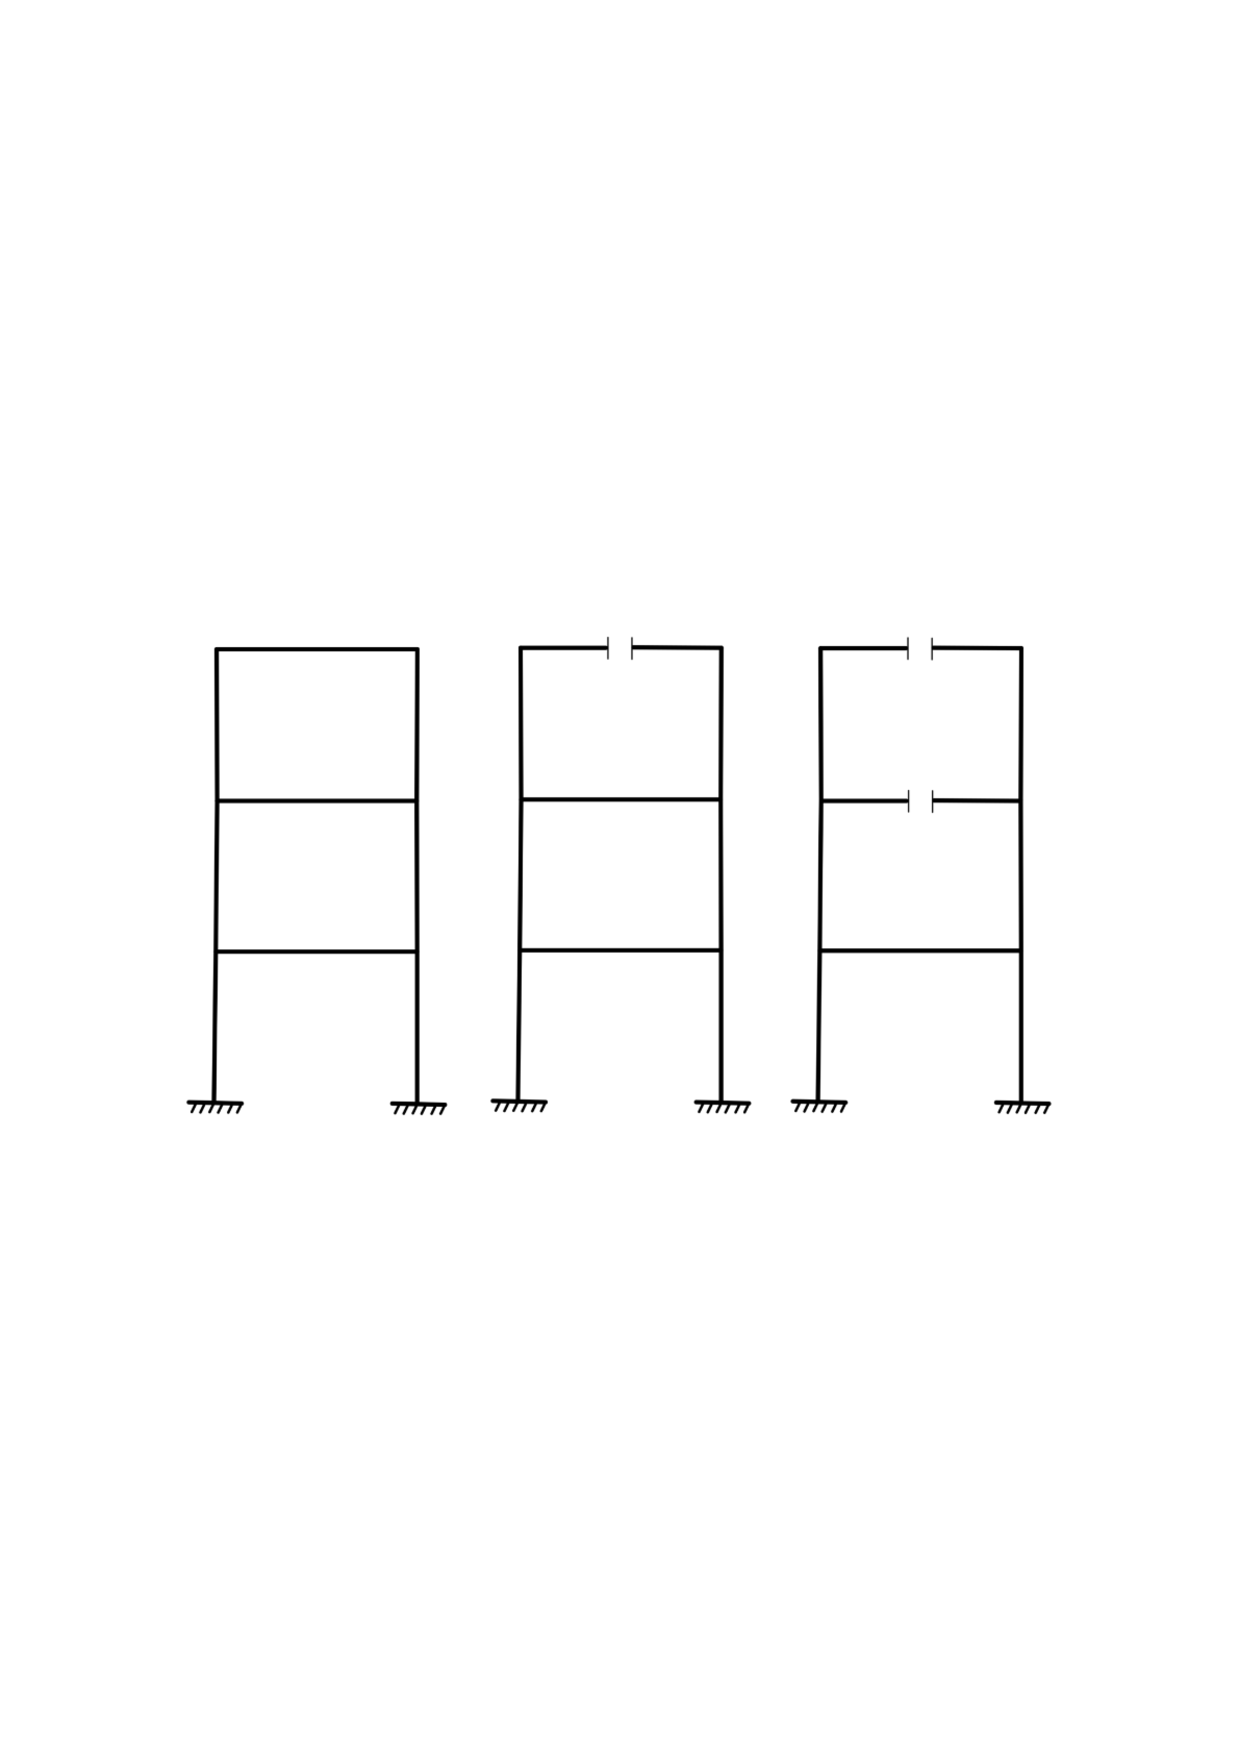
\includegraphics[scale=0.75]{cin_multipiano.pdf}
		\caption{Telaio a tre piani (schema ripreso nel
			Vol.~II per il caso deformabile): tre
			configurazioni con gradi di iperstaticità
			decrescenti. Da sinistra: tre maglie chiuse
			($\nu = -9$); taglio completo nella traversa
			superiore, due maglie chiuse ($\nu = -6$);
			tagli nelle traversi superiore e intermedia,
			una maglia chiusa ($\nu = -3$). Un terzo
			taglio aprirebbe l'ultima maglia ($\nu = 0$).}
		\label{fig:telaio_pluriconnesso}
	\end{figure}
